\documentclass[sn-basic]{sn-jnl}

% ---- compatibility shims (older sn-jnl.cls) ----
\providecommand{\jyear}[1]{}
\makeatletter
\@ifundefined{fnm}{\newcommand{\fnm}[1]{#1}}{}
\@ifundefined{sur}{\newcommand{\sur}[1]{#1}}{}
\@ifundefined{orgname}{\newcommand{\orgname}[1]{#1}}{}
\@ifundefined{orgaddress}{\newcommand{\orgaddress}[1]{#1}}{}
\@ifundefined{city}{\newcommand{\city}[1]{#1}}{}
\@ifundefined{country}{\newcommand{\country}[1]{#1}}{}
\@ifundefined{email}{\newcommand{\email}[1]{\texttt{#1}}}{}
\@ifundefined{orcid}{\newcommand{\orcid}[1]{#1}}{}
\makeatother
% ------------------------------------------------

\usepackage{pgfplots}
\pgfplotsset{compat=1.18}
\usepackage{pgfplotstable}
\usepackage{tikz}
\usepackage{booktabs}
\usepackage{mathtools}
\usepackage{amsmath,amssymb}

\providecommand{\state}{\textsc{state}}
\providecommand{\barrier}{\textsc{barrier}}

\title[Fractal/Entropic Programme]{The Fractal Nature of an Entropically-Driven Society: A Disciplined Structural Programme}

\author[1,2]{\fnm{Demetrios} \sur{Agourakis}\thanks{ORCID: 0000-0002-8596-5097; Email: \texttt{demetrios@agourakis.med.br}}}
\affil[1]{\orgname{Faculdade São Leopoldo Mandic}, \city{Campinas}, \country{Brazil}}
\affil[2]{\orgname{Pontifícia Universidade Católica de São Paulo (PUC-SP), Programa de Pós-Graduação em Biomateriais e Medicina Regenerativa}, \city{São Paulo}, \country{Brazil}}

\jyear{2025}

\abstract{
We propose a disciplined, testable account of “fractal/entropic” talk in social
explanation. A symbolic state $x$ represents coarse normative configurations
over claims and practices; dynamics follow an overdamped Langevin process on a
landscape $V(x)$ under agitation $D$ and exogenous inputs $u_t$. The associated
Fokker--Planck equation yields a stationary density $p^\star(x)\propto
e^{-V(x)/D}$ under detailed balance, while barrier-crossing rates follow
Kramers-like Arrhenius structure, $r\asymp A\,e^{-\Delta V/D}$, enabling
refutable predictions about dwell times, regime crossings, and shock responses.
We formulate a reviewer-facing stress test: (i) tail inference (power law vs.\
alternatives) with principled model comparison; (ii) small-world diagnostics in
interaction graphs; (iii) multifractal intermittency in behavioural/physiological
traces; (iv) misfit criteria and withdrawal conditions. A micro-case shows how
to register these diagnostics on public corpora. The framework is modest—agnostic
to microfoundations—yet empirically accountable via explicit keys, validity
domains, and falsification protocols.
}

\keywords{scientific representation; heavy tails; small-world networks; multifractals; Langevin; Fokker--Planck; Kramers rates; falsification}

\begin{document}
\maketitle

\section{Related work and novelty}\label{sec:related}
Our proposal intersects representation, idealization, heavy tails, and empirical
regularities in social systems, adopting a plural stance.

\textbf{Representation.} Inferential, key-based view \citep{Suarez2004,FriggHartmannSEP,Contessa2007}.
\textbf{Idealization.} Understanding under structured trade-offs \citep{Potochnik2017}.
\textbf{Heavy tails.} Disciplined tail inference with model comparison \citep{Newman2005,ClausetShaliziNewman2009,Mitzenmacher2004,Simon1955}.
\textbf{Empirical regularities.} Cities, firms, networks \citep{Zipf1949,Gabaix1999,Axtell2001,BarabasiAlbert1999}.
\textbf{Pluralism and structure.} Higher-level constraints with coexistence of models \citep{LadymanRoss2007,Wimsatt2007,Batterman2002}.

\emph{Novelty.} (i) An explicit \emph{representational key} for a normative landscape over symbolic states,
with misfit/withdrawal conditions; (ii) a falsification protocol that operationalizes when the analogy is warranted.

\section{Formal framework}\label{sec:formal}
\paragraph{State space.} $\Omega\subset\mathbb{R}^d$ collects coarse normative configurations. Keys map social to model predicates.
\paragraph{Dynamics.} Overdamped SDE
$\mathrm{d}X_t = -\nabla V(X_t)\,\mathrm{d}t + \sqrt{2D}\,\mathrm{d}W_t + u_t\,\mathrm{d}t$.
\paragraph{Fokker--Planck.} $\partial_t p = \nabla\!\cdot\!(p\,\nabla V) + D\,\Delta p$ with boundary conditions from the key.
\paragraph{Stationary density.} Under detailed balance, $p^\star(x) \propto \exp(-V(x)/D)$.
\paragraph{Kramers rate.} For double-well, $r \asymp A\,\exp(-\Delta V/D)$ \citep{Gardiner2009,Risken1996,Kramers1940}.

\paragraph{Invariants.} (i) Dwell concentration; (ii) exponential crossing sensitivity; (iii) transient currents under shocks; (iv) intermittency.

\section{Empirical programme and falsification}\label{sec:empirics}
\subsection{Tail inference}
Hill/MLE; KS bootstrap; Vuong non-nested tests \citep{ClausetShaliziNewman2009,Newman2005,Mitzenmacher2004,StumpfPorter2012}.
\emph{Withdrawal:} prefer alternatives $\Rightarrow$ remove power-law claim.

\subsection{Small-world diagnostics}
$C,L,\sigma$ with degree-preserving randomizations \citep{WattsStrogatz1998}. \emph{Withdrawal:} $\sigma\le1$.

\subsection{Intermittency}
$D_q$, $f(\alpha)$; MFDFA; surrogates \citep{KantzSchreiber2004}. \emph{Withdrawal:} multifractality unsupported.

\subsection{Shock assays}
Compare pre/post crossing intensities; test Arrhenius slope; \emph{Withdrawal:} insensitivity.

\noindent\textbf{Micro-case.}
\emph{SWOW} \citep{DeDeyne2019} and \emph{ZuCo} \citep{Hollenstein2018} used to instantiate the diagnostics.

\section{Registered analysis (plan)}\label{sec:regplan}
\paragraph{Hypotheses.} H1 Arrhenius; H2 $\sigma>1$; H3 intermittency near barriers; H4 disciplined tails \citep{ClausetShaliziNewman2009,Newman2005,StumpfPorter2012}.
\paragraph{Plan.} Randomizations for $\sigma$; KS/Vuong for tails \citep{Vuong1989}; shock-aligned crossing slopes; MFDFA+surrogates.
\paragraph{Withdrawal.} Any systematic failure $\Rightarrow$ local withdrawal; key re-registration.

\section*{Methods (summary)}
Tail pipeline; graph diagnostics; intermittency via MFDFA; sparse drift discovery; shock assays.

\section{Discussion and conclusion}\label{sec:conclusion}
The programme refrains from law-ascription yet upgrades “fractal/entropic” rhetoric to falsifiable structure.
Claims hold only under declared keys and domains; failures trigger withdrawal and re-registration.

\appendix
\section{Supplementary: Toy Empirics (inline)}\label{sec:supp-toy}

\subsection*{S1. Arrhenius/Kramers check}
\begin{figure}[!t]\centering
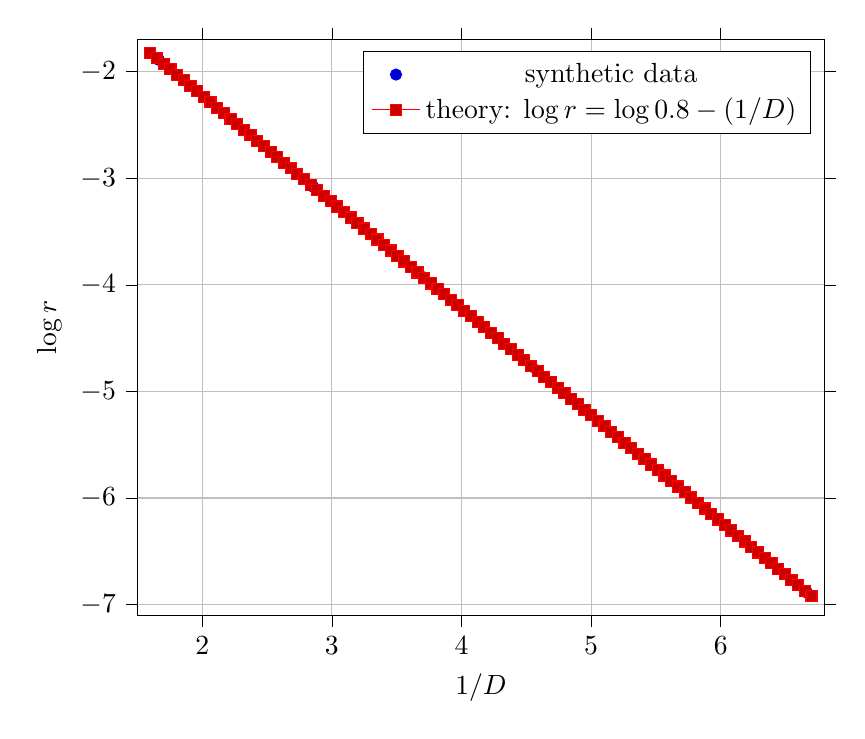
\begin{tikzpicture}
\begin{axis}[width=0.85\linewidth,xlabel={$1/D$},ylabel={$\log r$},xmin=1.5,xmax=6.8,ymin=-7.1,ymax=-1.7,grid=both,tick align=outside,tick style={black}]
\addplot+[only marks, mark=*, mark size=2pt]
table[row sep=\\]{x y \\ 6.6667 -6.889810218 \\ 5.5556 -5.778699107 \\ 4.5455 -4.768598097 \\ 3.7037 -3.926847255 \\ 2.8571 -3.080286408 \\ 2.2222 -2.445365774 \\ 1.6667 -1.889810218 \\ };
\addlegendentry{synthetic data}
\addplot+[domain=1.6:6.7, samples=100] {-0.223143551 - x};
\addlegendentry{theory: $\log r = \log 0.8 - (1/D)$}
\end{axis}
\end{tikzpicture}
\caption{Arrhenius plot (toy).}\label{fig:s1-arrhenius}
\end{figure}

\subsection*{S2. Rank--frequency}
\begin{figure}[!t]\centering
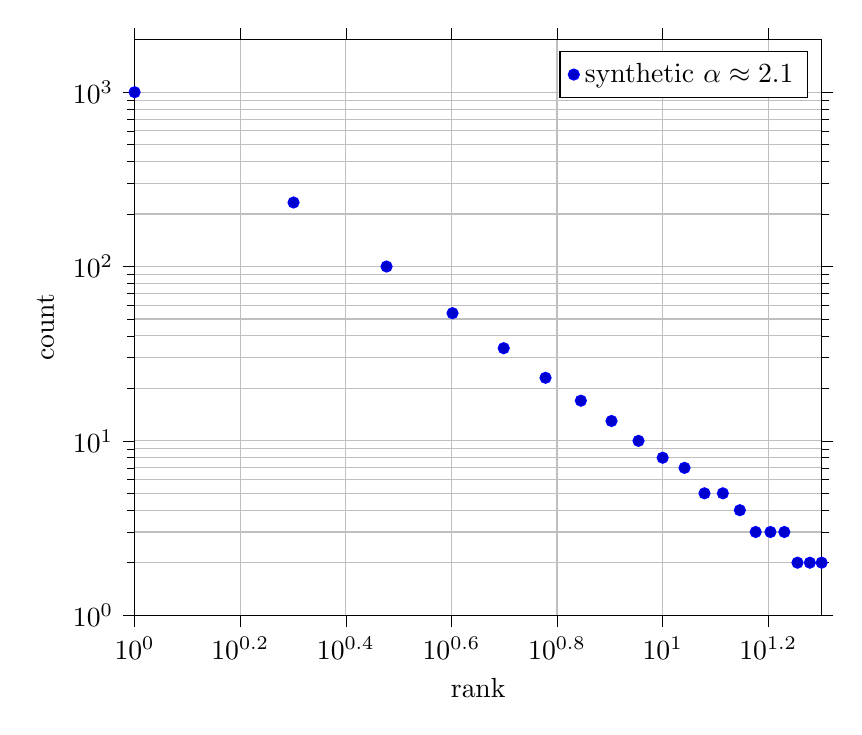
\begin{tikzpicture}
\begin{loglogaxis}[width=0.85\linewidth,xlabel={rank},ylabel={count},grid=both,tick align=outside,tick style={black},ymin=1,ymax=2000,xmin=1,xmax=20]
\addplot+[only marks, mark=*, mark size=2pt]
table[row sep=\\]{rank count \\ 1 1000 \\ 2 233 \\ 3 100 \\ 4 54 \\ 5 34 \\ 6 23 \\ 7 17 \\ 8 13 \\ 9 10 \\ 10 8 \\ 11 7 \\ 12 5 \\ 13 5 \\ 14 4 \\ 15 3 \\ 16 3 \\ 17 3 \\ 18 2 \\ 19 2 \\ 20 2 \\ };
\addlegendentry{synthetic $\alpha\approx 2.1$}
\end{loglogaxis}
\end{tikzpicture}
\caption{Rank--frequency (toy).}\label{fig:s2-rankfreq}
\end{figure}

\subsection*{S3. Dwell-time survival}
\begin{figure}[!t]\centering
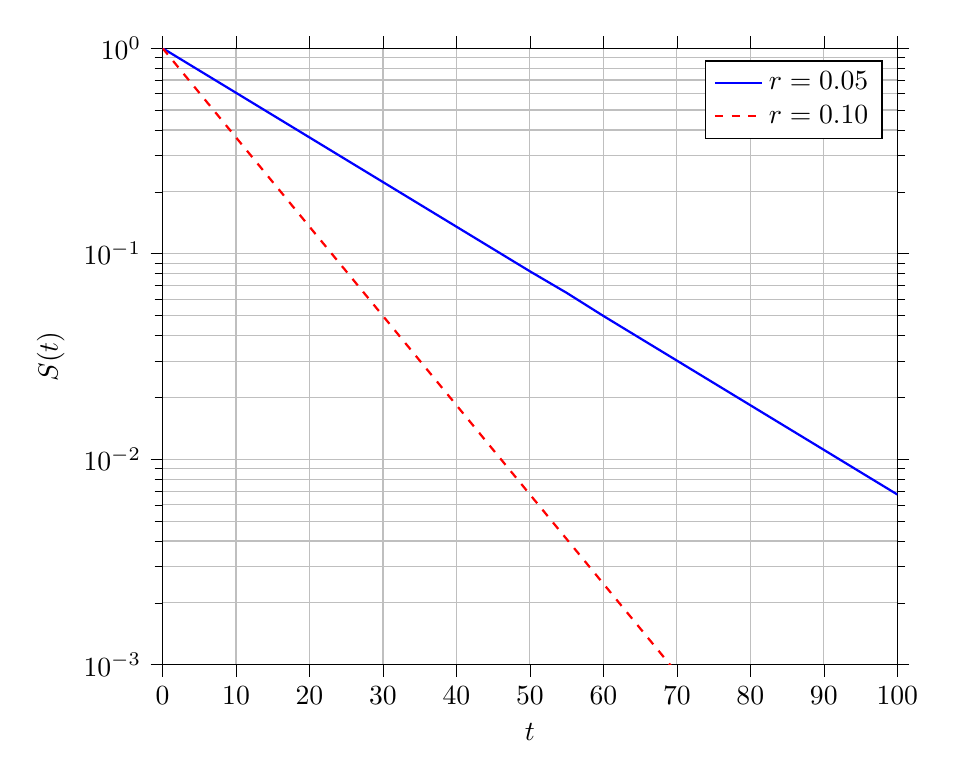
\begin{tikzpicture}
\begin{semilogyaxis}[width=0.90\linewidth,xlabel={$t$},ylabel={$S(t)$},grid=both,tick align=outside,tick style={black},xmin=0,xmax=100,ymin=1e-3,ymax=1]
\addplot+[no marks, thick]
table[row sep=\\]{t S \\ 0 1.0 \\ 5 0.7788007831 \\ 10 0.6065306597 \\ 15 0.4723665527 \\ 20 0.3678794412 \\ 25 0.2865047969 \\ 30 0.2231301601 \\ 35 0.1737739435 \\ 40 0.1353352832 \\ 45 0.1053992246 \\ 50 0.0820849986 \\ 55 0.0644936359 \\ 60 0.0497870684 \\ 65 0.0387742078 \\ 70 0.0301973834 \\ 75 0.0235177459 \\ 80 0.0183156389 \\ 85 0.0142642339 \\ 90 0.0111090000 \\ 95 0.00865 \\ 100 0.0067379470 \\ };
\addlegendentry{$r=0.05$}
\addplot+[no marks, thick, dashed]
table[row sep=\\]{t S \\ 0 1.0 \\ 5 0.6065306597 \\ 10 0.3678794412 \\ 15 0.2231301601 \\ 20 0.1353352832 \\ 25 0.0820849986 \\ 30 0.0497870684 \\ 35 0.0301973834 \\ 40 0.0183156389 \\ 45 0.011109 \\ 50 0.0067379470 \\ 55 0.0040867714 \\ 60 0.0024787522 \\ 65 0.0015034392 \\ 70 0.0009118820 \\ 75 0.0005530844 \\ 80 0.0003354626 \\ 85 0.0002034684 \\ 90 0.0001234098 \\ 95 0.0000742736 \\ 100 0.0000453999 \\ };
\addlegendentry{$r=0.10$}
\end{semilogyaxis}
\end{tikzpicture}
\caption{Dwell-time survival (toy).}\label{fig:s3-dwell}
\end{figure}

\bibliography{references_fos}
\end{document}
